\chapter{Scan Finder}
\label{ch:scanfinder}
This chapter describes \emph{Scan Finder}, an algorithm that can be used to retrieve all scanners position of a point cloud,  if there are any, regardless of its nature. Firstly, Section~\ref{sc:spec} reviews the context which brings this need and describes some characteristics of the expected solution. Then, Section~\ref{sc:work} reminds that there is no previous work related to this subject. Finally, Section~\ref{sc:highdens} describes a first step toward scanner location
finding before showing and discussing the results of two different approaches described respectively in Section~\ref{sc:grid-pattern} and Section~\ref{sc:elliptic}. To be clear, Section~\ref{sc:highdens} is a common first step to both methods.



\section{Specifications}
\label{sc:spec}
\subsection{Context}
\CC started to support point cloud reconstruction two (2) years ago. Today it even provides a hybrid processing mode which gives the opportuniy to combine the best of both words, photos and point clouds, in order to have a better precision. However, a recurring problem observed among \CC users is the impossibility to use the software after losing some metadata, specifically, scanners location. This is particulary problematic because usually, \CC users subcontract point cloud production to private companies which can charge them again for new exports (provided that they still have the point clouds). To enable customers to use their \emph{defective} point clouds, the graphic interface of \CC allows to specify a scanner location by hand by positioning it in a 3D representation of the point cloud. But, it does not work with merged scans; only one scanner location can be specified. Usually, users do not know the location and even if they know, the reconstruction is subjected to too much errors.

This is how the need for an algorithm to automatically find scanners positions in a point cloud is born. In addition, with such algorithm, \CC will have the possibility to enhance the set of supported file formats. Currently, it supports file formats such as \emph{PTX}, \emph{e57}, \emph{PLY}, \emph{POD}, each of them being able to store scanners positions. But not all file formats are able to do it. For instance, \emph{LAS} file format is not currently accepted as input because it does not provide any means of storing scanners location in metadata. Supporting more input file formats is also a good point of interest for \CC users.

\subsection{Objective}
In summary, the purpose here is to improve \CC point cloud support in two ways: support more file formats and allow users who lose scanners location to still use their point clouds. To do so, the algorithm must:
\begin{itemize}
  \item take as input any 3D point cloud captured from static scanners,
  \item be invariant to the number of scanners in the point cloud,
  \item be invariant to differences between scanners, such as: density, noise, rotation angle,
  \item find all scanners locations,
  \item have a reasonnable running time.
\end{itemize}

Let us emphasize here that as a first step, the algorithm is expected to work only with static point clouds. It would be difficult to have the same approach with static and mobile point clouds. Extending it to mobile point clouds is certainly the next step.



\section{Related Work}
\label{sc:work}
As said in the introduction, to the best of our knowledge, there have been no previous work on the subject.

\emph{``Detecting the positions of multiple scanners exclusively from a point cloud is a subject not identified as interesting by academics, and thus not tackled since this information is almost always available from the outset. The same holds true on the industry side, it is only recently that scanner position information is relevant for a few applications like \CC."}

The closest publications on the topic are \cite{ml1, ml2, ml3, ml4, ml5}. They use learning techniques to estimate the point of view of one particular photo based on other photos. But this belongs more to the photogrametry domain and therefore is not applicable in a point cloud context.



\section{Clustering high-density area}
\label{sc:highdens}
This section explains a common first step to methods described in Section~\ref{sc:grid-pattern} and Section~\ref{sc:elliptic}. For a better understanding, a quick introduction to LiDAR scanners is necessary.

\begin{figure}
  \centering
  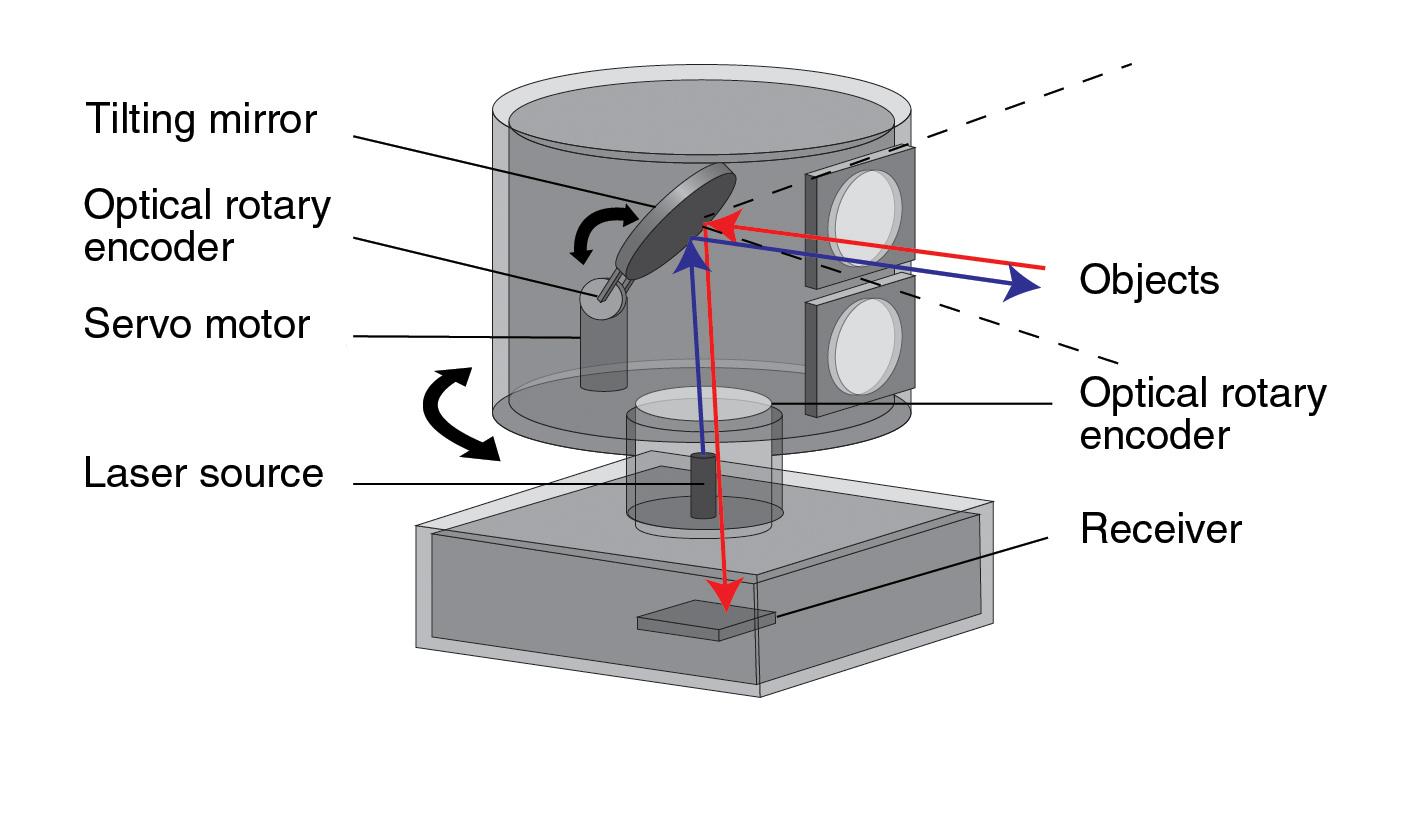
\includegraphics[scale=1]{img/lidar.jpg}
  \caption{Example of a LiDAR scanner.}
  \label{fig:lidar}
\end{figure}


\subsection{LiDAR scanner and context}
\label{subsc:lidar}
LiDAR is an acronym of Light Detection and Ranging. It is a remote sensing technology which uses the pulse from a laser to collect measurements. The principle is simple: it works in a similar way to Radar and Sonar but uses light waves from a laser, instead of radio or sound waves. A LiDAR system calculates how long it takes for the light to hit an object or surface and reflect back to the scanner and then, uses the velocity of light\footnote{The velocity, or speed of light is 299,792,458 metres
per second.} to calculate the distance. LiDAR systems can fire around 1,000,000 pulses per second. This paragraph is inspired by \cite{lidar}.

When scanning, there are two kind of rotations that a LiDAR scanner performs. They are indicated by black arrows in Figure~\ref{fig:lidar}. Not only a LiDAR scanner has a constant rotation angle when turning on itself but it also has a constant vertical rotation angle when scanning the environment. Because of these constant rotation angles, the further we go, the lower the point density is. On the contrary, the closer to the scanner we are, the higher the point density is. This density variation can be observed in
Figure~\ref{fig:density}. To conclude, extracting the most dense areas is interesting as they always are around scanner locations and then, reduce the global search area.

\begin{figure}
  \centering
  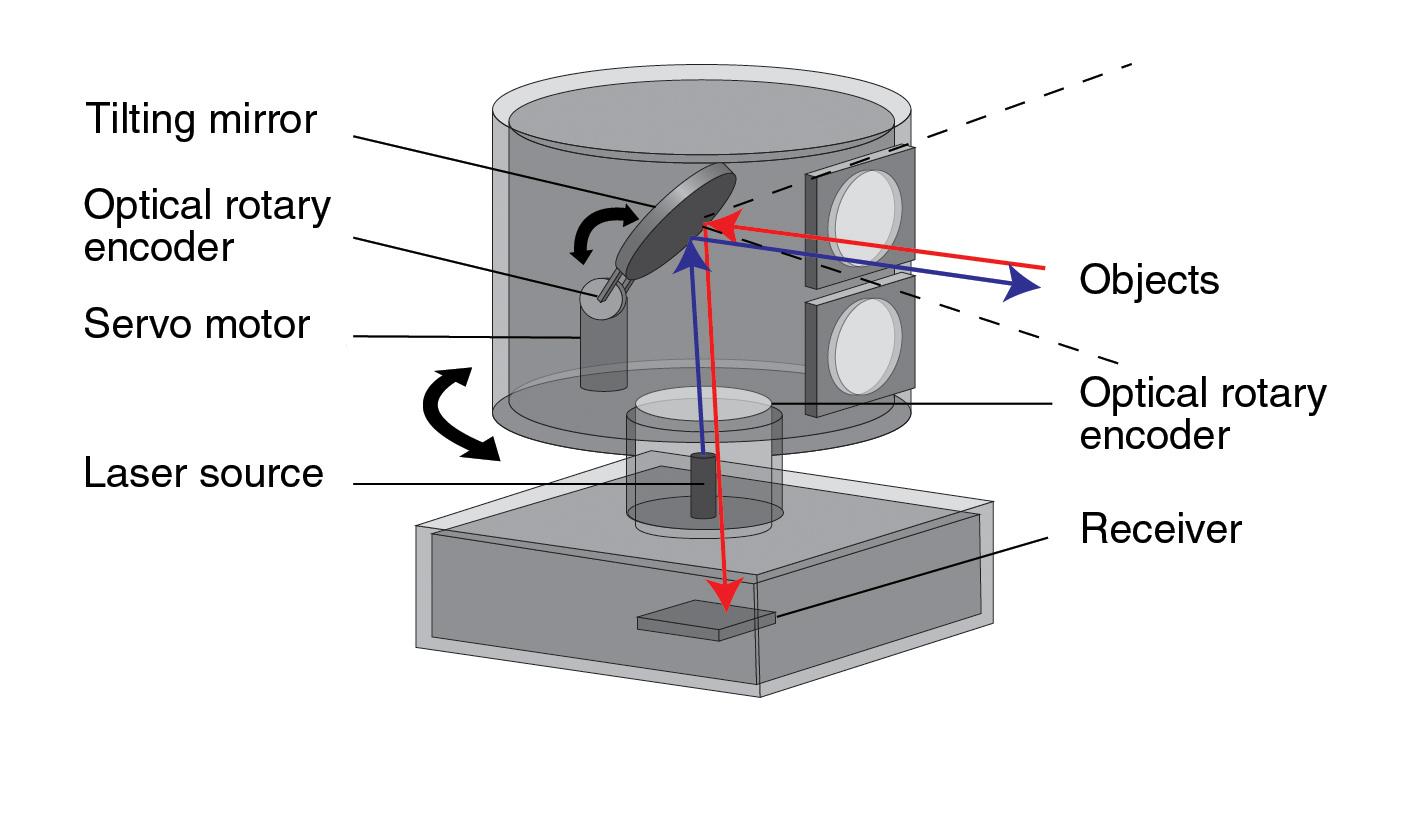
\includegraphics[scale=1]{img/lidar.jpg}
  \caption{Variation of density as we go further away from the source.}
  \label{fig:density}
\end{figure}


\subsection{Clustering and dense area extraction}
\label{subsc:highdens}
\begin{figure}
  \centering
  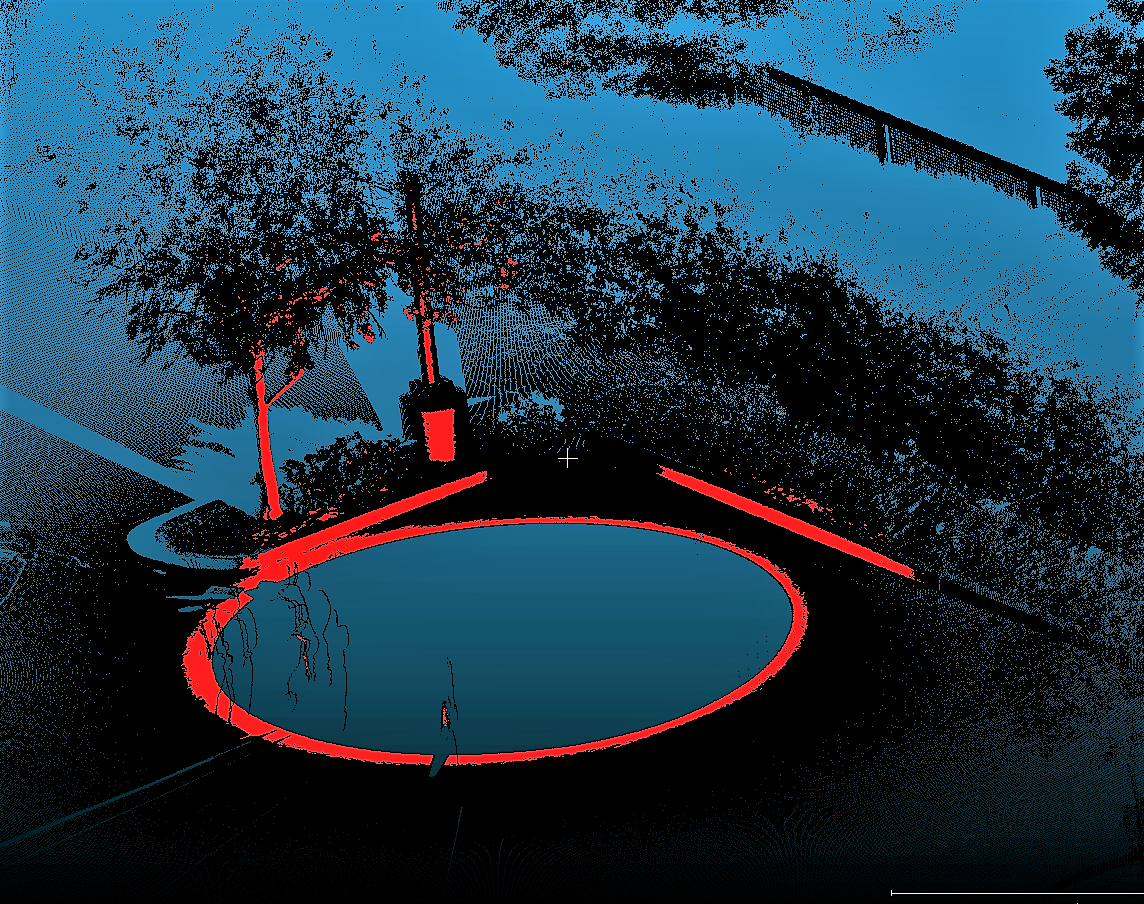
\includegraphics[scale=0.44]{img/highdens.png}
  \caption{The result of the high density extraction of a point cloud.}
  \label{fig:highdens}
\end{figure}

\begin{figure}
  \centering
  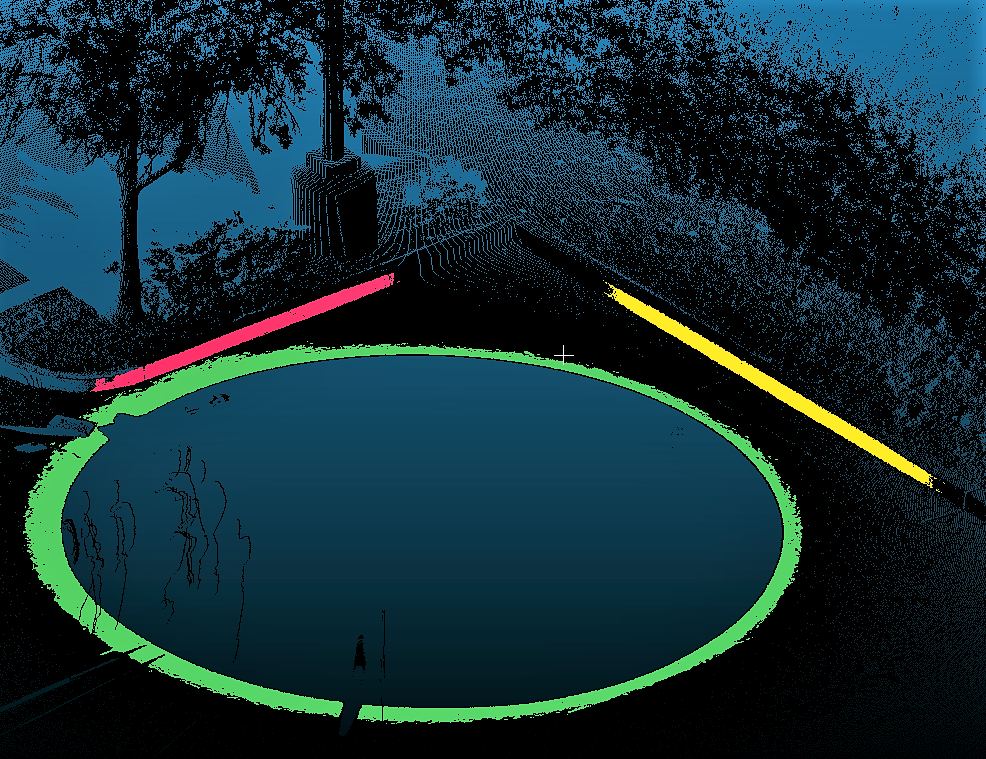
\includegraphics[scale=0.5]{img/cluster.png}
  \caption{The result after clustering dense points of a point cloud.}
  \label{fig:cluster}
\end{figure}

\begin{figure}
  \centering
  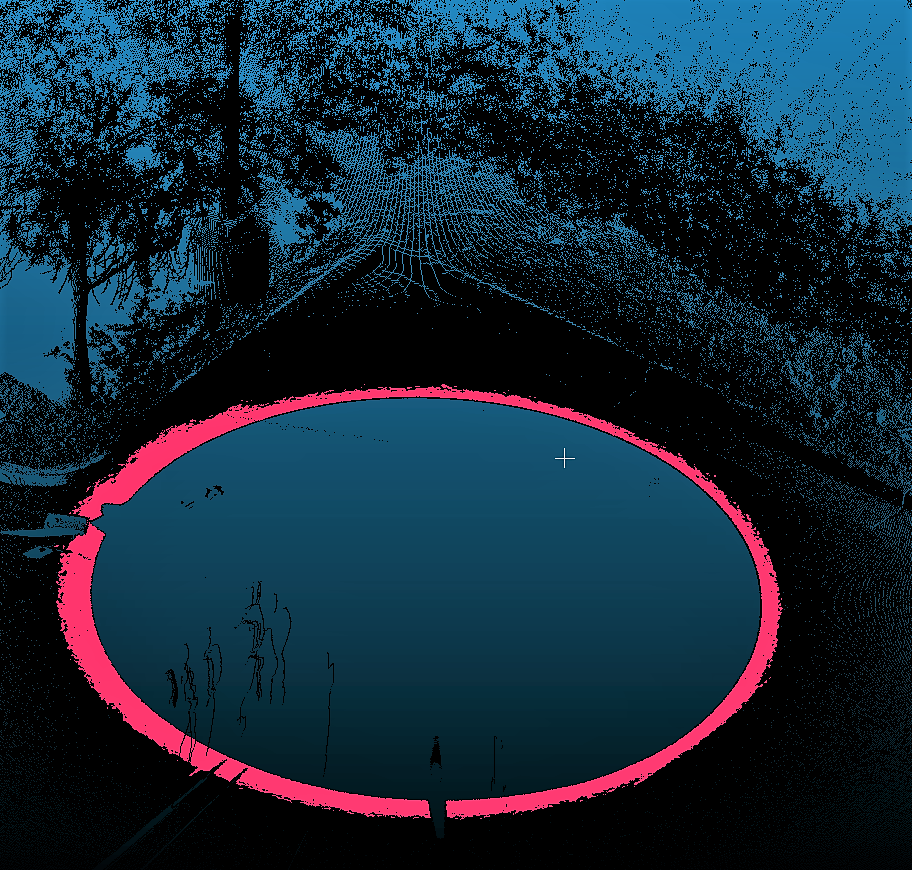
\includegraphics[scale=0.5]{img/circular.png}
  \caption{The result after trying to identify circular clusters.}
  \label{fig:circular}
\end{figure}

The first step of the algorithm is to detect high density regions in the point cloud. For each point, we compute its density based on the mean distance to its $k$ neighbors ($k \in [15,50]$). We extract high density regions by selecting a percentage of the densest points (percentage between 1 and 5\%). Figure~\ref{fig:highdens} shows some results of this high density point extraction. As you can see, they always contain the scanner. Note that the scanner is not able to scan below himself leading to an elliptic form\footnote{This elliptic form is the key point of the method described in Section~\ref{sc:elliptic}.} appearing in all point clouds.

Once these points are extracted, a clustering step is applied. The clustering is needed so that points from the point clouds corresponding to potentially different parts of the scene around the scanner can be separated. For each point, we compute its non-oriented normal and the associated \emph{confidence level} by performing a principal component analysis (PCA) on its local neighborhood. Section~\ref{subsc:pca} gives more details on how this PCA works. Then, as long as points are not attributed
to a cluster, we select the point on the flattest surface, and iteratively add its neighbors that share a coherent normal orienta-tion (the dot product of the two normals must be superior to 0.8 in our experiments). Note that the  flattest surface is determined using condifence levels, they tell which point belongs to a planar region. Figure~\ref{fig:cluster} shows the result of such clustering.

Once every point is clustered, we discard clusters with too few points (in our experiments, we use a threshold of 0.2\% of the number of high density points). We then detect clusters that are circular. A cluster is considered circular if its centroid, i.e. the average of all the points it contains, is far away from the points of the cluster. Figure~\ref{fig:circular} shows a circular cluster identified.

At this point, we have computed a coarse location of the scanner. Methods described in Section~\ref{sc:grid-pattern} and Section~\ref{sc:elliptic} use it in their own way in order to find scanner locations.



\section{The grid-pattern method}
\label{sc:grid-pattern}
This section explains one approach we tried in order to solve the problem. Before explaining the method in detail, let us first give the intuition behind this idea.

\subsection{Overview}
As said in Section~\ref{subsc:lidar}, LiDAR scanners perfom two kind of rotations. These constant vertical and horizontal rotation angles reveal some grid patterns on surfaces perpendicular to the ground\footnote{To be precise, perpendicular to the surface on which the scanner is installed.}. Figure~\ref{fig:grid1} shows an example of a grid pattern that can be found in point clouds. The purpose here is to find, for a single grid pattern, a relation between all constant rotation angles and the scanner's position. Therefore, this relation can be applied with all possible grid patterns in the point clouds, leading to a problem with a huge set of
constraints to solve. The idea is that only the real scanner's location is able to explain in the best way these constant rotation angles.

\begin{figure}[H]
  \centering
  
\includegraphics[scale=0.5]{img/grid1.png}
  \caption{Example of a grid pattern. As you can see there is a constant offset between each vertical line and each horizontal lines. Note that the offset between columns is not necessary the same than between lines.}
  \label{fig:grid1}
\end{figure}

This algorithm can be divided into two parts. The first step is to find \emph{accurate} grid patterns in point clouds. Once this is done, the second step is to build the equation that will be solved. These two parts are explained in the following subsections. Note that this approach does not work in multiscan mode, compare to the other approach described in Section~\ref{sc:elliptic}. It assumes there is only one scanner which explains all grid-patterns in the point cloud.

\subsection{Grid-pattern matching}
This subsection explains how to find \emph{accurate} grid patterns in point clouds in order to reduce as much as possible the noise and its impact during the problem resolution described in Section~\ref{subsc:eq}. A set of point is considered as an \emph{accurate} grid-pattern when:
\begin{itemize}
  \item it is planar as much as possible\footnote{Because of the noise.},
  \item the underlying planar surface is orthogonal to the surface of the ground,
  \item the gap between columns is consistent enough,
  \item the gap between lines is consistent enough.
\end{itemize}


\begin{algorithm}[tb]
  \SetAlgoVlined
  \DontPrintSemicolon
  \SetKw{Report}{report}
  \SetArgSty{}
  \SetKwFunction{GetPlanarPatches}{GetPlanarPatches}
  \SetKwProg{Fn}{Function}{}{}
  \Fn{\GetPlanarPatches{P}}{
    \KwIn{a pointcloud $P = \left\lbrace p_i \mid i \in [0, s]  \right\rbrace$.}
    \KwOut{a set of potential grid-pattern patches.}
    \tcc{We compute the normal of each point and keep both confidence level and normal $\left\langle \mu_i, \vec{v}_i \right\rangle$.}
    \tcc{See Section~\ref{subsc:pca} for more details on PCA algorithm.}
    \tcc{From here, $\forall i \in [0, s]$ we assume $\vec{v}_i$ to be the normal at $i$ and $\mu_i$ its confidence level.}
    \For{$i = 0;\ i < s;\ i = i + 1$}{
      $\left\langle \mu_i, \vec{v}_i \right\rangle \gets PCA($50 closest neighbours of $i)$\;
    }
    $R\gets\emptyset$\;
    visited $\gets\emptyset$\;
    \For{$i = 0;\ i < s;\ i = i + 1$}{
      \tcc{ Continue if already visited or is not planar enough.}
      \If{$i \in$ visited or $\mu_i > 0.001$}
      {\Continue}
      tmp $\gets \left\lbrace p_i \right\rbrace$\;
      \ForEach{$j \in $ 50 closest neighbours of $i$}{
        \tcc{If $\vec{v}_j$ and $\vec{v}_i$ are almost colinear and $j$ has not been seen yet.}
        \If{abs($\vec{v}_j \times \vec{v}_i$) $> 0.9$ and $j \not\in$ visited}{
          tmp $\gets$ tmp $\cup\ p_j$\;
          visited $\gets$ visited $\cup\ j$\;
        }
      }
      \tcc{If there is enough point for a grid-pattern patch.}
      \If{size of tmp $> 0.9\ \times$ 200}{
        $R \gets R\ \cup $ tmp
      }
    }
    \Return{$R$}\;
  }
  \caption{Find various not-overlaping planar patches in a point cloud.
    \label{alg:GetPlanarPatches}}
\end{algorithm}

Algorithm~\ref{alg:GetPlanarPatches} shows how to extract some planar patches in a point cloud. A preprocessing step already done and explained in Section~\ref{subsc:highdens} is to compute for each point of the point cloud, the normal and its \emph{confidence level}. This \emph{confidence level} plays a key role in the algorithm as it tells how planar the region around each point is. By browsing all points, each time we find a point with a good \emph{confidence level} ($> 0.001$), we start to build a patch around it. To do so, we extract its 50
closest neighbours and consider only those having their normal almost colinear to the normal of the starting point. If the size of the obtained set is bigger enough ($>\ 0.9 \times 200$), the set is kept and otherwise, not. Also, in order to avoid overlaping or patches too close, we keep track of visited points.

Although planar, this set of patches potentially contains: \textbf{(a)} patches whose underlying surfaces are not orthogonal to the surface of the ground and \textbf{(b)} patches without grid patterns. To filter out each \textbf{(a)} patch, we use a dot product between its normal and the normal of the circular cluster found in the high-density area\footnote{The circular cluster desribes the surface on which the scanner is positioned.} (see Section~\ref{sc:highdens}). For \textbf{(b)} patches,
the objectif is to indentify grid-patterns. To do so, we use least square method in order to fit lines. Least-square is explained in Section~\ref{subsc:least}. Fitting a line fall into linear least square problems. Figure~\ref{fig:fitline} shows how to fit a line to a set of points using the Eigen library~\cite{eigenweb}. The purpose is to use this line fitting in order to cluster lines and columns. Figure~\ref{fig:line-col-cluster} shows results of a clustering performed on two patches after several fittings and adjustements. We only keep firstly patches containing a grid-pattern and then, patches having a regular gap between columns and lines. The rest is discarded.

\begin{figure}
  \centering
  \begin{lstlisting}
    Eigen::VectorXf FitLine(std::vector<A3D::Point_3dPlus> const& points)
    {
      Eigen::MatrixXf mat(points.size(), 2);
      Eigen::VectorXf vec(points.size());
      int count = 0;
      for (auto it = points.begin(); it != points.end(); ++it)
      {
        mat(count, 0) = static_cast<float>(it->x());
        mat(count, 1) = static_cast<float>(it->y());
        vec(count++) = 1.0;
      }
      return mat.fullPivHouseholderQr().solve(vec);
    }
  \end{lstlisting}
  \caption{Function using least-square to fit a line to the given set of points.}
  \label{fig:fitline}
\end{figure}

\begin{figure*}[t!]
  \centering
    \begin{subfigure}[t]{0.5\textwidth}
      \centering
        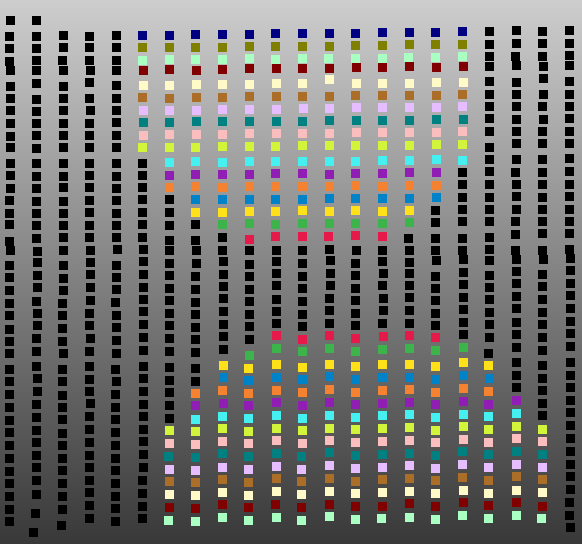
\includegraphics[height=2.5in]{img/grid-lines.png}
        \caption{Lines clustering performed on two patch.}
    \end{subfigure}%
    ~
    \begin{subfigure}[t]{0.5\textwidth}
      \centering
        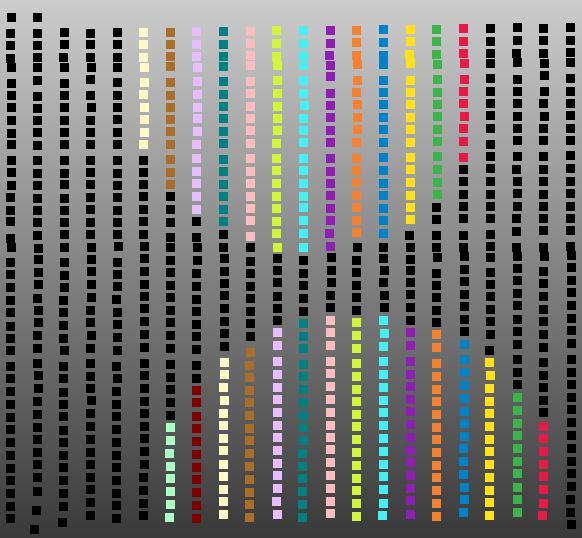
\includegraphics[height=2.5in]{img/grid-cols.png}
        \caption{Column clustering performed on two patches.}
    \end{subfigure}
    \caption{Example of columns and lines clustering in order to identify grid-patterns.}
    \label{fig:line-col-cluster}
\end{figure*}

Once only \emph{accurate} patches are kept, columns and lines are identified, the problem can be formalised.

\subsection{Equation to solve}
\label{subsc:eq}

For a little recall of Section~\ref{sc:grid-pattern}, the purpose here is to find a relation between the scanner's position (what we are looking for) and the regular gaps between lines and columns. Again, the gap between lines and the gap between columns is not necessary the same. Also, at this point, we already have a reduced area of research which is arround the circular cluster obtained in Section~\ref{subsc:highdens}. What we want, is a set of equations that will help
to set the point within this area.

Look at Figure~\ref{fig:topview}. There are four (4) vertical lines viewed from a bird's eye: $a$, $b$, $c$ and $d$. They are represented as points because of the point of view. The regular gap between those lines is represented by the relation $d_1 = d_2$. But instead of working on the regular gap distance, one can work with the regular rotation angle of the scanner. These angles directly involve the scanner location in all equations. Here is how the problem is built: for each grid-pattern, and for
each pair of two consecutive lines (or columns), we minimize the absolute difference between their respective angles (here $\alpha_1$ and $\alpha_2$). This is a non-linear least-square problem.

FIXME: More explanation?

\begin{figure}
  \centering
  \begin{tikzpicture}
    \draw[fill] (0,0) circle (2pt) coordinate (a) node[above=0.2cm]{$a$};
    \draw[fill] (2.5,0) circle (2pt) coordinate (b) node[above=0.2cm]{$b$};
    \draw[fill] (5,0) circle (2pt) coordinate (c) node[above=0.2cm]{$c$};
    \draw[fill] (7.5,0) circle (2pt) coordinate (d) node[above=0.2cm]{$d$};
    \draw[fill] (3.75, -4.5) circle (2pt) coordinate (e) node[below=0.1cm,black]{$s$};
    \draw[red, <->, shorten <= 0.2cm, shorten >= 0.2cm]
      (a) -- node[above]{$d_1$} (b);
    \draw[red, <->, shorten <= 0.2cm, shorten >= 0.2cm]
      (c) -- node[above]{$d_2$} (d);
    \draw[dashed] (a) -- (e) -- (b)
      pic["$\alpha_1$", draw=red, red, solid, <-, angle eccentricity=1.2,
          angle radius=1cm] {angle=b--e--a};
    \draw[dashed] (c) -- (e) -- (d)
      pic["$\alpha_2$", draw=red, red, solid, <-, angle eccentricity=1.2,
          angle radius=1cm] {angle=d--e--c};
  \end{tikzpicture}
  \caption{A top view over four (4) vertical grid lines ($a$, $b$, $c$ and $d$) and a scanner ($s$).}
  \label{fig:topview}
\end{figure}

\subsection{Results and discussions}
\begin{figure}
  \centering
  \begin{tikzpicture}
    \draw[fill] (0,0) circle (2pt) coordinate (a) node[above=0.2cm]{$a$};
    \draw[fill] (2.5,0) circle (2pt) coordinate (b) node[above=0.2cm]{$b$};
    \draw[fill] (5,0) circle (2pt) coordinate (c) node[above=0.2cm]{$c$};
    \draw[fill] (7.5,0) circle (2pt) coordinate (d) node[above=0.2cm]{$d$};
    \draw[fill] (3.75, -4.5) circle (2pt) coordinate (e) node[below=0.1cm,black]{$s$};
    \draw[fill] (-4, 0) circle (2pt) coordinate (f) node[below=0.1cm,black]{$s'$};
    \draw[red, <->, shorten <= 0.2cm, shorten >= 0.2cm]
      (a) -- node[above]{$d_1$} (b);
    \draw[red, <->, shorten <= 0.2cm, shorten >= 0.2cm]
      (c) -- node[above]{$d_2$} (d);
    \draw[dashed] (a) -- (e) -- (b)
      pic["$\alpha_1$", draw=red, red, solid, <-, angle eccentricity=1.2,
          angle radius=1cm] {angle=b--e--a};
    \draw[dashed] (c) -- (e) -- (d)
      pic["$\alpha_2$", draw=red, red, solid, <-, angle eccentricity=1.2,
          angle radius=1cm] {angle=d--e--c};
    \draw[dashed, blue] (a) -- (f) -- (b)
      pic["$\alpha_1'$", draw=blue, blue, above, solid, <-, angle eccentricity=1.2,
          angle radius=1cm] {angle=b--f--a};
    \draw[dashed, blue] (c) -- (f) -- (d)
      pic["$\alpha_2'$", draw=blue, blue, below, solid, <-, angle eccentricity=1.2,
          angle radius=1cm] {angle=d--f--c};

  \end{tikzpicture}
  \caption{Illustration of the problem preventing the grid-pattern method from finding the scanner location. Not that this is a top view over four (4) vertical grid lines ($a$, $b$, $c$ and $d$), the apprixmation ($s'$) and the real scanner ($s$).}
  \label{fig:grid-problem}
\end{figure}

\begin{figure}[H]
  \centering
  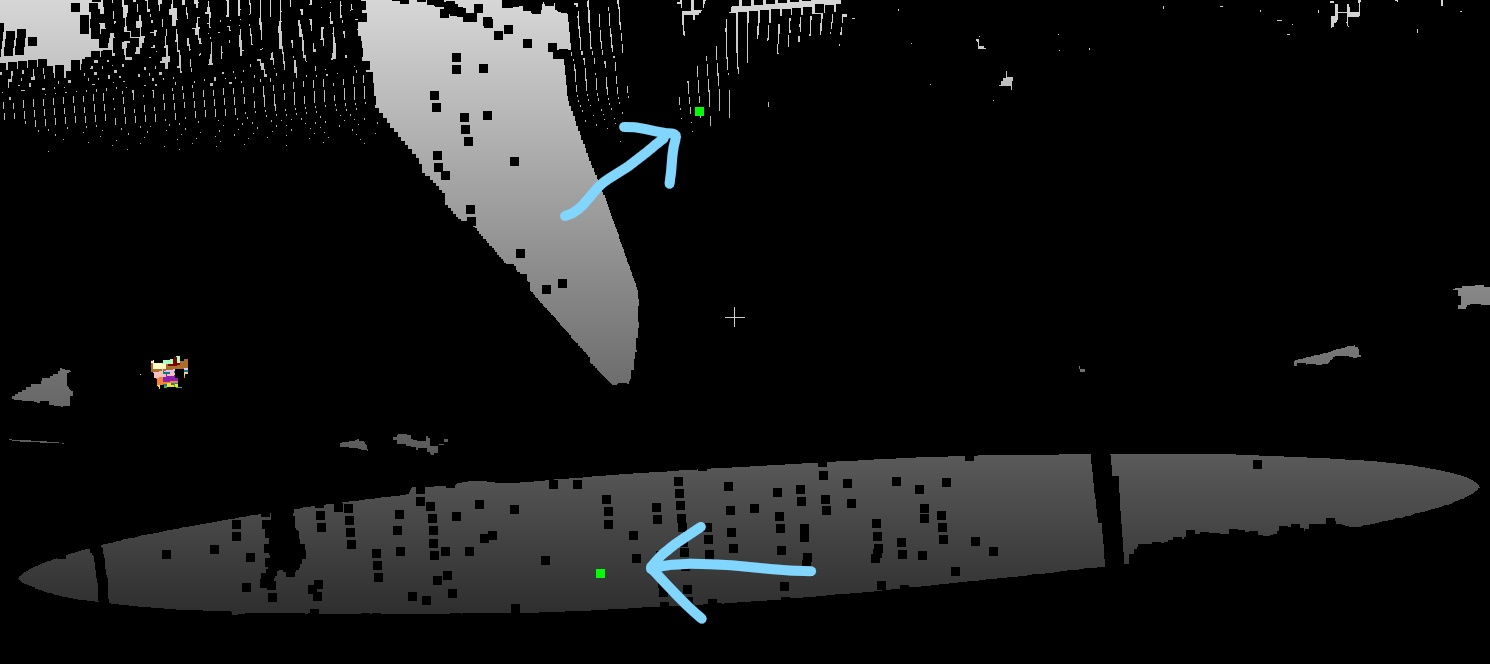
\includegraphics[scale=0.3]{img/grid-result.jpg}
  \caption{An approximation of the scanner location using the grid-pattern method. The real scanner location is highlighted by the upper arrow while the approximation is highlighted by the lower one.}
  \label{fig:grid-result}
\end{figure}

Figure~\ref{fig:grid-result} shows a result of grid-pattern approximation of scanner location. This method does not perform quite well. One would think that the approximation is not far from the real scanner location but reducing the area of research to a cube arround the circular cluster can be misleading. We tried to remove the area constraints and observed that the approximation moves entirely away from the real location and even the point cloud itself. It can stoop pretty low, go to really
high altitude, on the left, on the right. It completely depends on the distribution of the grid-patterns in the point cloud.

Let us take one grid-pattern in order to illustrate the problem: Figure~\ref{fig:grid-problem}. As our method tries to minimize the differences between all pairs of angles, here $\alpha_1$ and $\alpha_2$, the ideal case is if the scanner location belongs to the underlying surface of the grid-pattern. Here, $\alpha_1'$ and $\alpha_2'$ are perfectly equal: $\alpha_1' - \alpha_2' = 0$. Therefore, with a huge set of equations involving several grid-patterns, the optimal solution for
the solver is to put the scanner in the underlying surface of the \emph{mean plan of all grid-pattern underlying planes}. This is why, without the reduced area constraint, the approximated scanner is far away from the point cloud as the solver tries to reduce all angle differences and then, satisfy all grid-patterns.

To conclude, angles differences are not discriminating enough. We believe there is a way to express the problem in another way, in order to bypass this behaviour but we deciced to try another approach presented in Section~\ref{sc:elliptic}. In addition, this approach is limited to one scanner whereas the other method works with multiple scaners.



\section{The elliptic method}
\label{sc:elliptic}

\subsection{Overview}


\subsection{Fitting ellipse}
\begin{figure}[h]
  \centering
  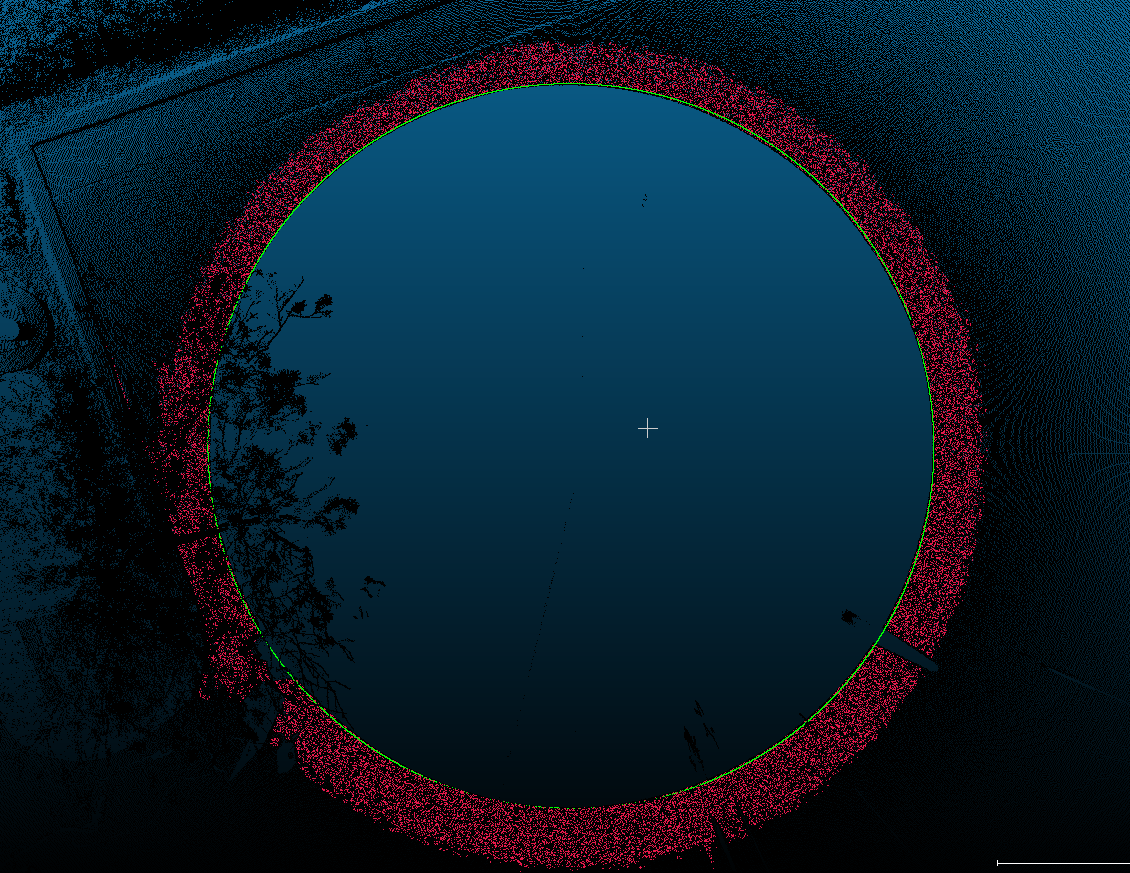
\includegraphics[scale=0.4]{img/ellipse.png}
  \caption{Ellipse fitted on a circular cluster.}
  \label{fig:ellipse}
\end{figure}

For each of the circular cluster, we extract the points close to the inside of the cluster and then fit an ellipse using a least-square algorithm.

FIXME: Explain ellipse fitting (refere to ransac and least square in background).

The center of the fitted ellipse is computed, and the center of the scanner lies on the z-axis passing through this center. This is only an approximation that suppose that the ground is approximately horizontal. This approximation applies to a vast majority of cases where terrestrial scanning is used. If needed, a refinement of the horizontal position of the scanner can be obtained by applying the same process as described below to estimate the vertical position of the scanner.

\subsection{Equation to solve}
To estimate the height of the scanner, we will use the slight variation in density of the points in the circular cluster. The intuition is that the density of a local point is linked to its distance from the scanner. Using multiple points, we are able to triangulate the position of the scanner. For a point $p$ in the high density circular cluster, we note $r$ the distance between the scanner and the point, $d$ the density of the point, and $\alpha$ the angle between the normal of the point and the direction
from the point of the scanner. Using the fact that point density decreases proportionally as moving away from the scanner, the following relation should be verified for any pair of points.
\begin{equation}
\frac{d_a \times r_a^2}{\cos(\alpha_a)} = \frac{d_b \times r_b^2}{\cos(\alpha_b)}
\end{equation}
where $d_a$ is the density of $a$ and $d_b$ the density of $b$. This is explained in Figure~\ref{fig:sideview}.

For each circular cluster, we pick a sample of N points (in our experiments, N=6 points) with different densities. We then use a non-linear least square solver to determine the position of the scanner, mixing together   equations (15 if N=6). As a result, we retrieve an estimated position of the scanner location.

\begin{figure}
  \centering
  \begin{tikzpicture}[scale=0.8]
    \draw[fill] (-8.2,0) circle (0pt) coordinate (p1);
    \draw[fill] (6.5,0) circle (0pt) coordinate (p2);
    \draw[gray, thin] (p1) -- node[near end, right=3cm]{ground level} (p2);

    \draw[fill] (0,0) circle (0pt) coordinate (x) node[above=0.2cm]{};
    \draw[fill] (5,0) circle (0pt) coordinate (y) node[above=0.2cm]{};
    \draw[fill,blue] (5.5,0) circle (2pt) coordinate (a) node[below=0.2cm]{$a$};
    \draw[fill,red] (-2,0) circle (2pt) coordinate (b) node[below=0.2cm]{$b$};
    \draw[fill] (5.5,2) circle (0pt) coordinate (c);
    \draw[fill] (-2,2) circle (0pt) coordinate (d);
    \draw[black, dashed, <->, line width=0.5mm] (x) -- node[below=-0.1cm]{ellipse} (y);
    \draw[blue](a) circle [radius=4.05];
    \draw[red](b) circle [radius=5.2];
    \draw[fill] (2.45,2.7) circle (4pt) coordinate (s) node[right=0.2cm]{$s$};
    \draw[dashed, blue] (s) -- node[near start, right]{$r_a$} (a) -- (c)
      pic["$\alpha_a$", draw=blue, blue, solid, <-, angle eccentricity=0.8,
          angle radius=1cm] {angle=c--a--s};
    \draw[dashed, red] (d) -- (b) --  node[near end, left=0.1cm]{$r_b$} (s)
      pic["$\alpha_b$", draw=red, red, solid, <-, angle eccentricity=0.8,
          angle radius=1cm] {angle=s--b--d};
    \draw[red, <-, line width=0.3mm] (d) -- node[left, near start]{$\vec{n}_b$}(b);
    \draw[blue, <-, line width=0.3mm] (c) -- node[right, near start]{$\vec{n}_a$}(a);
  \end{tikzpicture}
  \caption{A side view of the ellipse and two spheres intersecting at the scanner position $s$ and their respective centers $a$ and $b$. We have the relation $\frac{d_a \times r_a^2}{\cos(\alpha_a)} = \frac{d_b \times r_b^2}{\cos(\alpha_b)}$ where $d_a$ is the density of $a$ and $d_b$ the density of $b$.}
  \label{fig:sideview}
\end{figure}


\subsection{Results and discussions}
\begin{figure}[h]
  \centering
  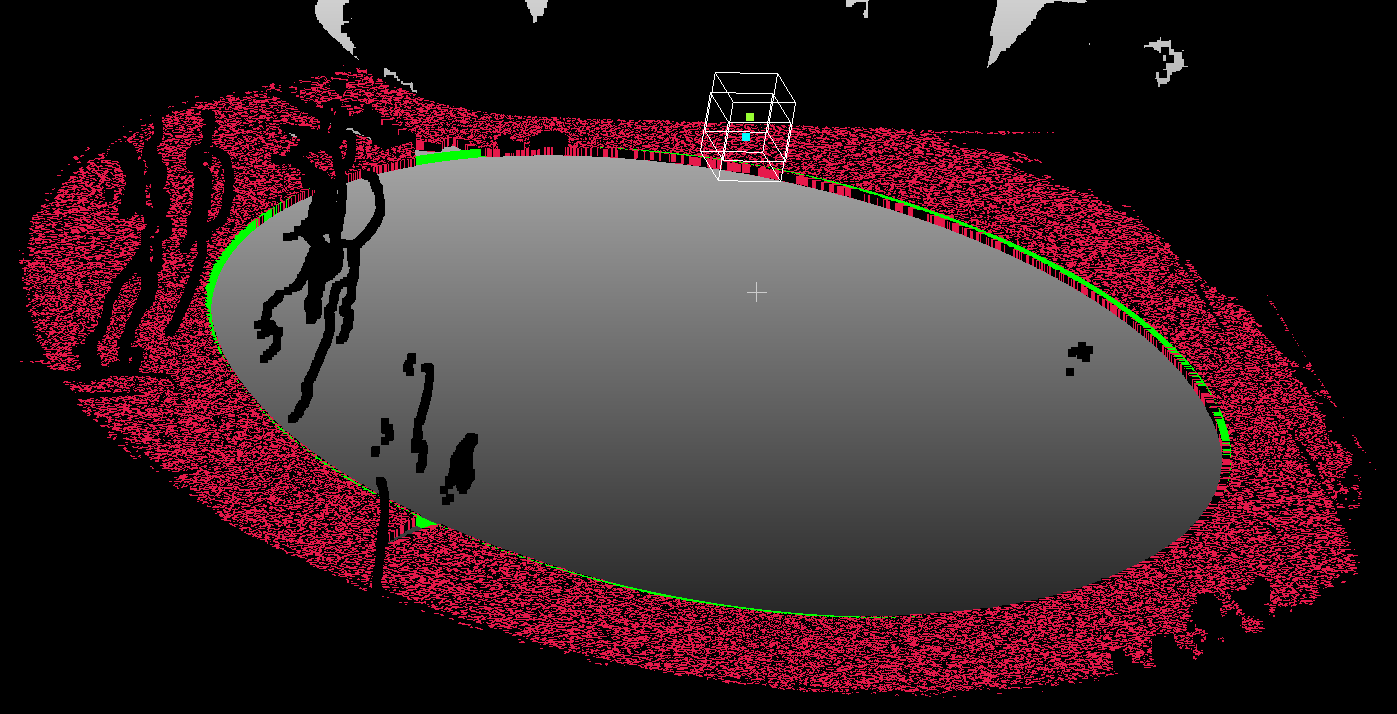
\includegraphics[scale=0.4]{img/ellipse-result.png}
  \caption{Light blue point in the box is the correct position, green point next to it is our estimation.}
  \label{fig:ellipse-result}
\end{figure}
\begin{figure}[h]
  \centering
  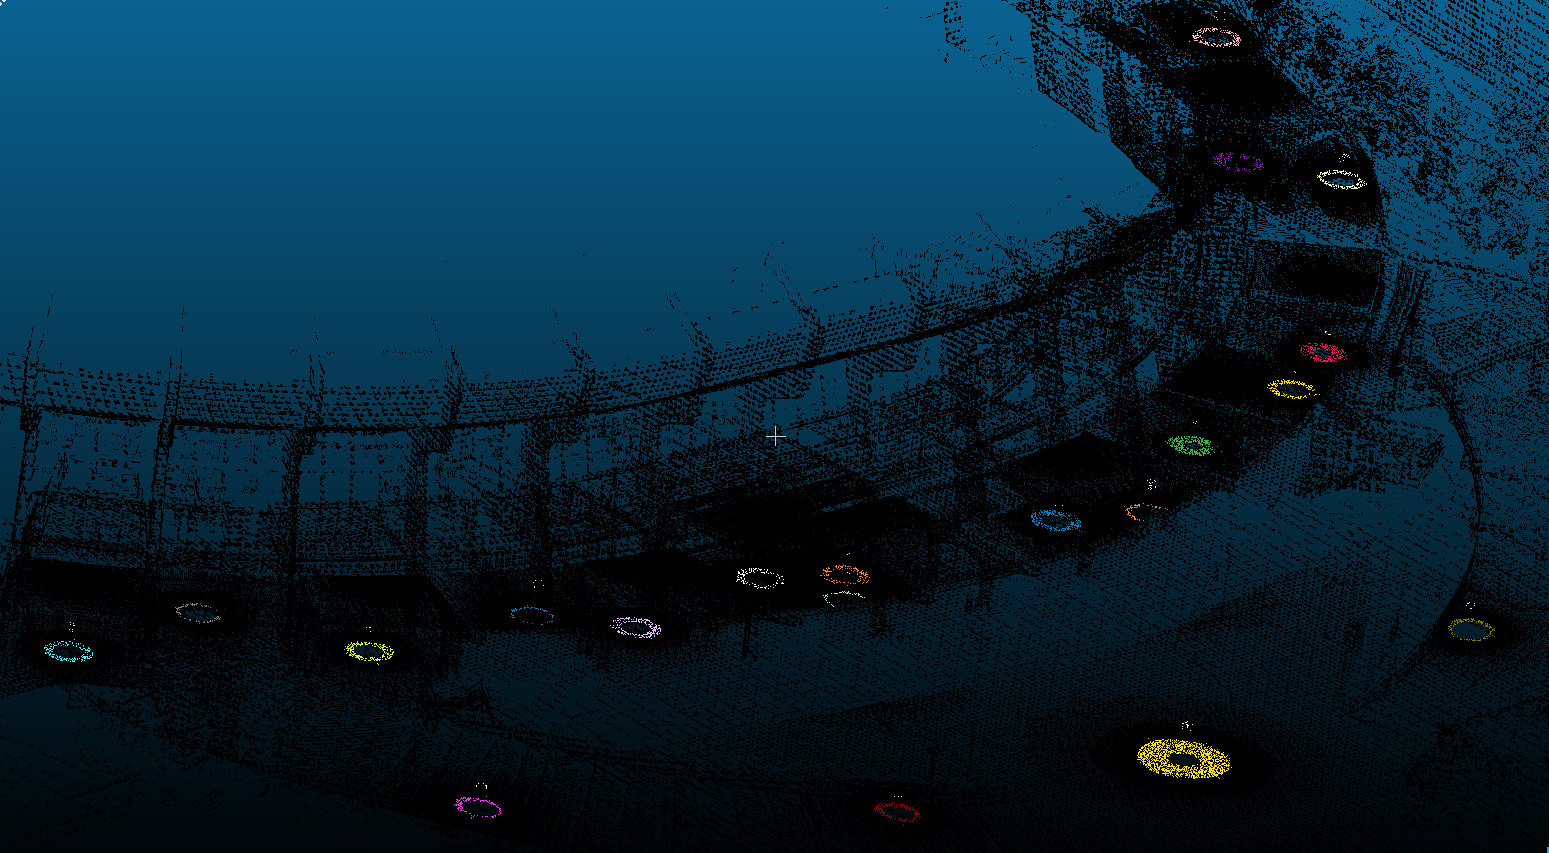
\includegraphics[scale=0.3]{img/ellipse-multi1.png}
  \caption{Multiple locations detected in a large point cloud.}
  \label{fig:ellipse-multi1}
\end{figure}
\begin{figure}[h]
  \centering
  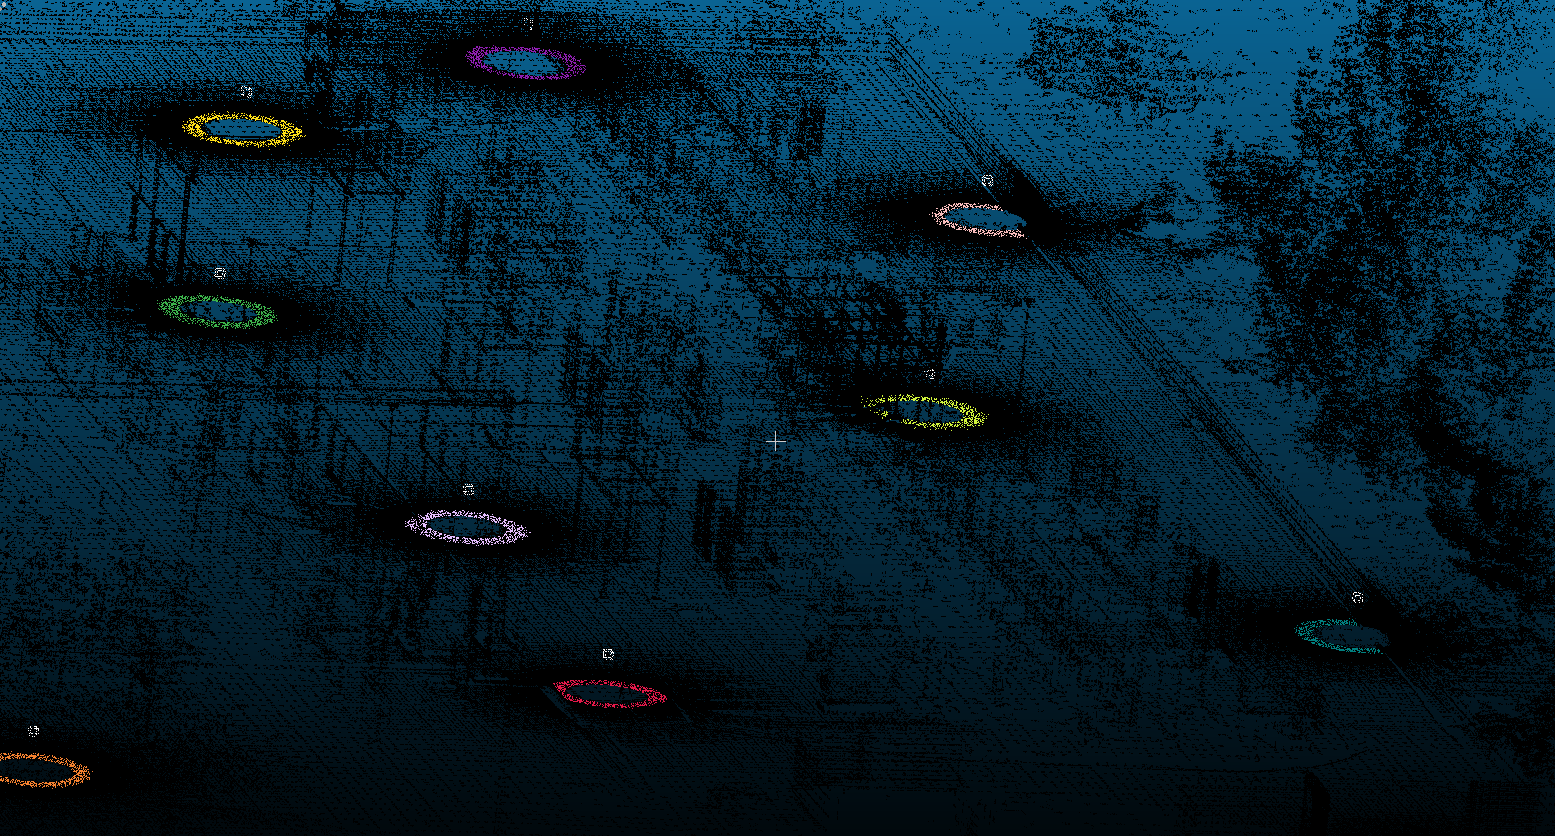
\includegraphics[scale=0.3]{img/ellipse-multi2.png}
  \caption{Multiple locations detected in another large point cloud.}
  \label{fig:ellipse-multi2}
\end{figure}

Testing on various reference datasets, we found that the error between the correct position and our estimation ranges between 2 and 20 cm.

This pipeline is particularly suited for multi-scan point clouds. Terrestrial scanners tend to generate most of the points close to their positions. If we consider that scans are not taken in the same close vicinity, high density clusters are disjoint. We confirm with hypothesis in our experiments. Therefore, the coarse detection works well in the multi-scan hypothesis. The same idea applies for the fine position algorithm: most points in the circular cluster come from a single scanner. The few other points coming from different scanners don’t have a significant impact on the local density of the points. That way, the scanner height is correctly detected in a multi-scan setting.
